%\documentclass{beamer}
\documentclass[handout]{beamer}
%\usepackage{beamerthemesplit} // Activate for custom appearance
\usetheme{Boadilla}
\newtheorem{Proposition}[theorem]{Proposition}%
\newcommand{\BP}{\mathbf{P}}
\newcommand{\BE}{\mathbf{E}}
\newcommand{\BI}{\mathbf{1}}


\setbeamertemplate{theorems}[numbered]

\title{STAT 7200}
 \subtitle{Introduction to Advanced Probability \newline Lecture 9}
\author{Taylor R. Brown}
\institute{}
\date{}

\begin{document}

\frame{\titlepage}

\section[Outline]{}
\frame{\tableofcontents
``A First Look at Rigorous Probability Theory" (Jeffrey Rosenthal) Sections 4.1 and 4.2 }



\section{Foundations of Probability}


\subsubsection{Expectations of Simple Random Variable}

\frame
{
  \frametitle{Expectations of Simple Random Variable}

   \begin{itemize}


                         \item<1-> Over a probability triple $(\Omega,\mathcal{F}, \BP)$, if we have an indicator random variable $\BI_A$ on $A\in \mathcal{F}$, so that $\BI_A=1$ when $\omega\in A$, and $\BI_A=0$ when $\omega \not \in A$. Then we can define expectation of this indicator random variable as: $\BE(\BI_A)=\BP(A)$.
                         
\item<2-> Similarly, we can extend this definition to \textit{simple random variables}. A  random variable $X$ is simple if it only takes a finite number of values. If we list the possible values that $X$ may take as $x_1, x_2,\cdots, x_n$, we should be able to represent $X$ as: $X=\sum_{i=1}^n x_i \BI_{A_i}$, where $A_1, A_2,\cdots, A_n$ forms a partition of $\Omega$. 
                                                  

\item<3-> Then we define the expectation of simple random variable as: $\BE(X)=\sum_{i=1}^n x_i \BP(A_i)$.

\end{itemize}
}

\frame
{
  \frametitle{Property of Expectations: Linearity}

   \begin{itemize}


\item<1-> \textbf{Linearity} The expectation of a simple random variable is linear. That is, for two simple random variables $X, Y$ and $a,b \in \mathbf{R}$, we have $\BE(aX+bY)=a\BE(X)+b\BE(Y)$.
                         
\item<2-> \textbf{Proof}: Let us denote $X=\sum_{i=1}^n x_i \BI_{A_i}$ and $Y=\sum_{j=1}^m y_j \BI_{B_j}$. Since $\{A_i\}$ forms a partition of $\Omega$, $\{B_i\}$ forms a partition of $\Omega$, $\{A_i\cap B_j\}$ also forms a partition of $\Omega$. Then $aX+bY=\sum_{i=1}^n a x_i \BI_{A_i}+\sum_{j=1}^m b y_j \BI_{B_j}=\sum_{i=1}^n \sum_{j=1}^m  (a x_i+b y_j)  \BI_{A_i \cap B_j}$. 
                                                  
\item<3->[-] So 
\begin{align*}
\BE(aX+bY)& =\sum_{i=1}^n \sum_{j=1}^m  (a x_i+b y_j)  \BP(A_i \cap B_j) \\ & =\sum_{i=1}^n  a x_i \left[\sum_{j=1}^m \BP(A_i \cap B_j)\right]+ \sum_{j=1}^m  b y_j \left[ \sum_{i=1}^n \BP(A_i \cap B_j) \right] \\ &=\sum_{i=1}^n  a x_i \BP(A_i )+ \sum_{j=1}^m  b y_j \BP(B_j)=a\BE(X)+b\BE(Y)
\end{align*}
                                                  
                             
                    \end{itemize}
}



\frame
{
\frametitle{Property of Expectations: Others}

\begin{itemize}

\item<1-> \textbf{Consequence of Linearity} By linearity of expectation, for $X=\sum_{i=1}^n x_i \BI_{A_i}$ where $A_1, \cdots A_n$ may not form a partition of $\Omega$, we still have  $\BE(X)=\sum_{i=1}^n x_i \BP(A_i)$.
                         

\item<2-> \textbf{Order Preserving} The expectation of simple random variable preserves the order, that is, for simple random variables $X, Y$, if $X\leq Y$ for every $\omega$, then we have $\BE(X)\leq \BE(Y)$.
                         
\item<3-> \textbf{Proof}: This property is quite obvious since $X\leq Y$ implies $Y-X\geq 0$, then $\BE(Y-X)\geq 0$ and we have $\BE(X)\leq \BE(Y)$.
                                                                                                                           
\item<4-> A direct consequence of order preservation is the \textbf{triangle inequality}: since $-|X|\leq X\leq |X|$, we have $|\BE(X)|\leq \BE(|X|)$.     
                                                          

\item<5-> \textbf{Functions of Simple Random Variables} Suppose $X$ is simple random variable $X=\sum_{i=1}^n x_i \BI_{A_i}$. Given any function $f:\mathbf{R}\rightarrow \mathbf{R}$, $f(X)=\sum_{i=1}^n f(x_i) \BI_{A_i}$ is also a simple random variable and $\BE(f(X))=\sum_{i=1}^n f(x_i) \BP(A_i)$.
                                                                                                                                 \end{itemize}
}


\frame
{
  \frametitle{Expectation and Independence}

   \begin{itemize}


\item<1-> \textbf{Expectation and Independence} If $X, Y$ are simple random variables and $X\bot Y$, then $\BE(XY)=\BE(X)\BE(Y)$.                         
\item<2-> \textbf{Proof}: Denote $X=\sum_{i=1}^n x_i \BI_{A_i}$ and $Y=\sum_{j=1}^m y_j \BI_{B_j}$, and without loss of generality, suppose $\{x_i\}$ are distinct and $\{y_j\}$ are distinct. 
                                                  
\item<3->[-] Since $X\bot Y$, $\BP(X=x_i, Y=y_j)=\BP(X=x_i)\BP(Y=y_j)$, then we have $\BP(A_i\cap B_j)=\BP(A_i)\BP(B_j)$
                                                                                                    
\item<4->[-] $XY=\sum_{i=1}^n \sum_{j=1}^m  x_iy_j \BI_{A_i \cap B_j}$ is a simple random variable and   
\begin{align*}
\BE(XY)&=\sum_{i=1}^n \sum_{j=1}^m  x_iy_j \BP(A_i \cap B_j) \\ 
&= \sum_{i=1}^n \sum_{j=1}^m  x_iy_j \BP(A_i)\BP(B_j) \\ 
&= \left[\sum_{i=1}^n  x_i \BP(A_i )\right] \left[ \sum_{j=1}^m  y_j \BP(B_j) \right]=\BE(X)\BE(Y)
\end{align*}
                                                                                                                           
\end{itemize}
}

\subsubsection{Expectations of Non-Negative Random Variables}


\frame
{
\frametitle{Expectations of Non-Negative Random Variables}

\begin{itemize}


\item<1-> For a non-negative random variable $X$, we define its expectation as the supremum of all the expectations of the simple random variables $Y$ not greater than $X$. That is:
                         
$$\BE(X)=\sup\{\BE(Y): Y\text{ is simple}, Y\leq X\}$$


\begin{figure}[h!]
  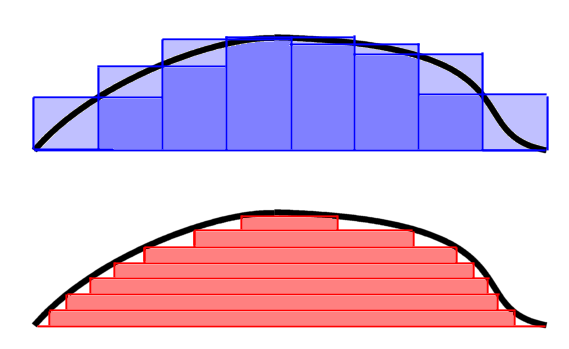
\includegraphics[width=76mm]{RandLintegrals.png}
  \caption{$Y \leq X$, $X$ is nonnegative, and $Y$ is simple and nonnegative}
\end{figure}





\end{itemize}
}

\frame
{
\frametitle{Expectations of Non-Negative Random Variables}

$$\BE(X)=\sup\{\BE(Y): Y\text{ is simple}, Y\leq X\}$$


\begin{itemize}

\item<2->First, this definition does not contradict the definition for simple random variables since $\BE(X)=\sup\{\BE(Y): \text{Y } simple, Y\leq X\}$ if $X$ is simple.
 
\item<3->Second, this definition still preserves orderings: If $X_1$ and $X_2$ are two non-negative random variables so that $X_1\leq X_2$, then $\BE(X_1)\leq \BE(X_2)$. 

\item<4-> Example: $E[X^k] < \infty \implies E[X^{k-1}] < \infty$ because $x^{k-1} \le \max(x^k,1) \le 1 + x^k$

\item<5->Third, the expectation might be infinite. Example: $X(\omega) = \sum_{n=1}^{\infty} 2^n 1(2^{-n} \le \omega < 2^{-(n-1)})$ on $([0,1], \mathcal{F}, \BP)$

\item<6-> Proving linearity requires another result...

\end{itemize}
}


\frame
{
  \frametitle{The Monotone Convergence Theorem}

\begin{itemize}

\item<1->[]
\begin{Theorem}[The Monotone Convergence Theorem] 
If $X_1, X_2, \ldots$ are non-negative random variables such that $\{X_n\} \nearrow X$. Then $X$ is a random variable and $\lim_{n\rightarrow \infty} \BE(X_n)=\BE(X)$. 
\end{Theorem}

\item<2->[]
$\{X_n\} \nearrow X$ means $X_1 \le X_2 \le \ldots$ and $\lim_{n \to \infty} X_n(\omega) = X(\omega)$.

\end{itemize}

Proof on next slide...
}

\frame
{
  \frametitle{The Monotone Convergence Theorem}

\begin{itemize}

\item<1->[]
\begin{Proof} 
For any real $x$, $\{X \le x\} = \cap_n \{X_n \le x\}$, so the limit of random variables is still a rv. 
\newline

By order preservation, $\BE[X_n] \le \BE[X]$ for all. Taking the limit yields $\lim_{n \to \infty} \BE[X_n] \le \BE[X]$. The limit exists because it is a monotonic sequence, and it may be infinite.
\newline

Last, pick $Y = \sum_{i=1}^m y_i 1_{A_i}$ be a simple rv such that $Y \le X$ and such that $\{A_i\}$ partitions $\Omega$. Pick an $0 <\epsilon$, and for each $i$, define $A_{in} = \{\omega \in A_i : X_{n}(\omega) \ge y_i - \epsilon  \}$ (not a partition). Clearly $\{A_{in}\} \nearrow A_i$ for any $i$. For a fixed $n$, $\BE[X_n] \ge  \sum_{i=1}^m (y_i - \epsilon) \BP(A_{in}) = \sum_{i=1}^m y_i \BP(A_{in}) - \epsilon \BP(\cup_{i=1}^m A_{in})$. Taking the limit: $\lim_{n \to \infty} \BE[X_n] \ge \sum_{i=1}^m y_i \BP(A_{i}) - \epsilon$. This is true for any epsilon, and any simple random variable $Y \le X$, and so the result holds.

\end{Proof}

\end{itemize}
}

\frame
{
  \frametitle{The Monotone Convergence Theorem}

You can't always move the limit inside and outside of the expectation operator.
\newline

Example, on $([0,1],\mathcal{F},\BP)$ consider $X_n(\omega) = n 1_{(0,n^{-1})}$.
\newline

% Also, you can replace the condition $\{X_n\} \nearrow X$ with $\{X_n\} \nearrow X$ almost surely.
}


\frame
{
\frametitle{Non-Negative Random Variables as a Limit of Simple Random Variables}

\begin{itemize}

\item<1->[-] Given any non-negative random variable $X$, we will construct a sequence of simple random variable $\Psi_n(X)$, such that the expectation of  $\Psi_n(X)$ would approach the expectation of $X$.
                         
\item<2->[-]  To construct $\Psi_n(X)$, for each $n$:
                          
\item<2->[-]  If $X\geq n$, $\Psi_n(X)=n$ . 
                         
\item<3->[-]  When $X<n$, we divide the region $[0,n)$ evenly into $n 2^n$ intervals.
\begin{itemize}
\item For instance, if $n=1$, we will divide $[0,1)$ into $[0,1/2), [1/2,1)$; 
\item If $n=2$, we divide $[0,2)$ into $[0,1/4), [1/4, 1/2),\cdots, [7/4, 2)$). 
\end{itemize}
                         
\item<4->[-]  If $k/2^n\leq X< (k+1)/2^n$ ($0\leq k\leq n2^n-1$),  $\Psi_n(X)=k/2^n$.                    
                                
\item<5-> This definition ensures that 1) $\Psi_n(X)$ is simple, as it only takes at most $n2^n+1$ different values; 2) $\Psi_n(X)\leq X$; 3) $\Psi_n(X)$ forms a sequence of increasing random variables, and 4.) $\Psi_n(x)\rightarrow x$ as $n\rightarrow \infty$. 
                                                                                                                                 \end{itemize}
}





\frame
{
  \frametitle{Property of Expectations of Non-Negative Random Variables }

   \begin{itemize}


                         
\item<1-> As $\Psi_n(X)\rightarrow X$ as $n\rightarrow \infty$, by the monotone convergence theorem, we have $\lim_{n\rightarrow \infty} \BE(\Psi_n(X))=\BE(X)$. Then we may prove the following properties for non-negative random variables based on the similar properties for simple random variables.

\item<2->  \textbf{Linearity} For non-negative random variables $X, Y$, and $a, b>0$, we have $\BE(aX+bY)=a\BE(X)+b\BE(Y)$.

\item<3->[]\textbf{Proof} We may construct $\Psi_n(X)\rightarrow X$ and $\Psi_n(Y)\rightarrow Y$, then $a\Psi_n(X)+b\Psi_n(Y)$ is an increasing sequence of non-negative random variables that converge to $aX+bY$. By the monotone convergence theorem:

\item<4->[]
\begin{align*}\BE(aX+bY)& =\lim_{n\rightarrow \infty} \BE (a\Psi_n(X)+b\Psi_n(Y)) \\ 
& =\lim_{n\rightarrow \infty}[ a\BE(\Psi_n(X))+b\BE(\Psi_n(Y)) ]=a\BE(X)+b\BE(Y)
\end{align*}

\end{itemize}
}




\frame
{
  \frametitle{Property of Expectations of Non-Negative Random Variables }

   \begin{itemize}



                         
                                                  \item<1->  \textbf{Expectation and Independence} For non-negative random variables $X\bot Y$, we have $\BE(XY)=\BE(X) \BE(Y)$. ( $\Psi_n(X)$ is a function of $X$, $\Psi_n(Y)$ is a function of $Y$, then if $X\bot Y$, $\Psi_n(X)\bot \Psi_n(Y)$) 
                                                  
                                                  
                                                                           \item<2->\textbf{Proof} We may construct $\Psi_n(X)\rightarrow X$ and $\Psi_n(Y)\rightarrow Y$, then $\Psi_n(X)\Psi_n(Y)$ are an increasing sequence of non-negative random variables that converge to $XY$.  Furthermore, as $\Psi_n(X)$ is a function of $X$, $\Psi_n(Y)$ is a function of $Y$, then if $X\bot Y$, $\Psi_n(X)\bot \Psi_n(Y)$.
                                                                           
                                                                           
                                                                   \item<3->[-]          By the monotone convergence theorem:
                                                         \begin{align*}\BE(XY)& =\lim_{n\rightarrow \infty} \BE (\Psi_n(X)\Psi_n(Y)) \\ & =\lim_{n\rightarrow \infty}[ \BE(\Psi_n(X)) \BE(\Psi_n(Y)) ]=\BE(X)\BE(Y)\end{align*}


                                                  
                              
                                                  
                                 \end{itemize}
}



\end{document}
